% \subsection{OpenTelemetry}
% \label{subsec:opentelemetry}

Es haben sich auf Basis dieser drei Grundpfeiler einige Technologien entwickelt. Jedoch sind die meisten Ansätze proprietär und nicht miteinander kompatibel, weswegen das Bedürfnis einer Standardisierung entstand. OpenTracing, OpenCensus \cite{OpenCensus} sowie OpenTelemetry \cite{OpenTelemetry} sind aus dieser Bewegung stammende Standards, die darauf abzielen herstellerunabhängige Observability-Konzepte zu definieren.

OpenTelemetry (OTel) ist ein sich derzeit\footnote{Ein erster (General-Availability-)Release der Spezifikation ist für die erste Hälfte 2021 geplant \cite{OpenTelemetryGARelease} (Stand 01.03.2021)} entwickelnder Standard, welcher als Ziel hat, dass das Erfassen, Weiterleiten und Verarbeiten von  Tracing-, Metrik- und Logdaten\footnotemark{} herstellerunabhängig ermöglicht wird. OTel entwickelte sich aus dem Zusammenschluss der Teams hinter den beiden Standards OpenTracing und OpenCensus, die das gleiche Ziel der Vereinheitlichung, der hier existierenden Ansätze, verfolgen  \cite{UseNixDistributiveTracing}. Weiterhin versucht OTel nicht nur die bisherige Landschaft zu vereinigen, sondern definiert bspw. eine zukunftsorientierte Architektur aus unterschiedlichen Komponenten und wie diese miteinander kommunizieren \cite{DistributedTracingInPractice}. Microsoft, Google, führende Unternehmen und Entwickler von Observability-Technologien sowie die die Cloud-Native-Computing-Foundation (CNCF) arbeiten an der Entwicklung des OTel Standards \cite{DistributedTracingInPractice} \cite{OpenTelemetryCommunityMembers}.

\nomenclature[Fachbegriff]{OTel}{OpenTelemetry}
\nomenclature[Fachbegriff]{CNCF}{Cloud-Native-Computing-Foundation}
\footnotetext{Die Entwicklung einer Logging-Spezifikation ist im Gange \cite{OpenTelemetryLoggingSpecification}.}

Der OpenTelemetry-Standard definiert einige Komponenten, die jeweils spezielle Aufgabengebiete erfüllen und standardisiert mit anderen Komponenten kommunizieren. Die Komponenten werden nachfolgend näher erklärt anhand des Beispiels eines Tracing-Spans sowie der \autoref{fig:otel-components}.

\begin{itemize}
	\item \textbf{API}: Die API stellt die öffentlich sichtbare Schnittstelle der OTel-Verarbeitung (des SDKs) dar, Verwender sind Entwickler sowie instrumentierende Bibliotheken. Mit der API kann ein Entwickler einen Trace initialisieren, darauf aufbauend einen Span erzeugen und diesen Span starten.
	\item \textbf{Instrumentation-Library}: Bei einer solchen Bibliothek handelt es sich um eine spezifische Anbindung der OTel-API an bspw. ein Framework (wie JAX-RS oder Angular). Teilweise erlauben solche Bibliotheken auch eine automatische Erfassung der Daten, sodass bspw. bei relevanten Methoden (wie Schnittstellaufrufen) ein Span erzeugt wird.
	\item \textbf{SDK}: Das SDK stellt das Herzstück der Verarbeitung bei OTel dar und pflegt u. A. die Beziehung zwischen den Spans sowie reicht diese an Verarbeitungsmethoden weiter und letztendlich übergibt sie an die exportierende Komponente. Der erzeugte Span wird mit seinen Kontextinformationen im SDK vorgehalten und bei Beendigung des Spans wird dieser an die angebunden Exporter übergeben.
	\item \textbf{Exporter}: Exporter sind spezifische Anbindungen, die Daten im OTel-Format annimmt und diese für die Gegenstelle aufbereitet sowie an diese transportiert. Die Gegenstelle kann entweder eine Datensenke darstellen, oder auch eine weiterverarbeitende Komponente sein. In diesem Beispiel wird der Span nicht in ein anderes Format überführt, da er an einen OTel-Colletor gesendet wird.
	\item \textbf{Collector}: Collector sind eine OTel-Schnittstelle um unterschiedliche OTel-Daten anzunehmen und diese an weitere Systeme mithilfe von Exporter zu überreichen. Bei dem Exporter in diesem Beispiel werden die Daten in das passende Format des Telemetry-Backends überführt.
	\item \textbf{Telemetry-Backend}: Ein Telemetry-Backend stellt die Datensenke der OTel-Daten dar und bietet den Entwicklern und Betreibern eine Visualisierung der gesammelten Daten. Beispiele hierfür sind z. B. Jaeger \cite{Jaeger} oder Prometheus \cite{Prometheus}.
\end{itemize}
 
\begin{figure}[H]
	\centering
	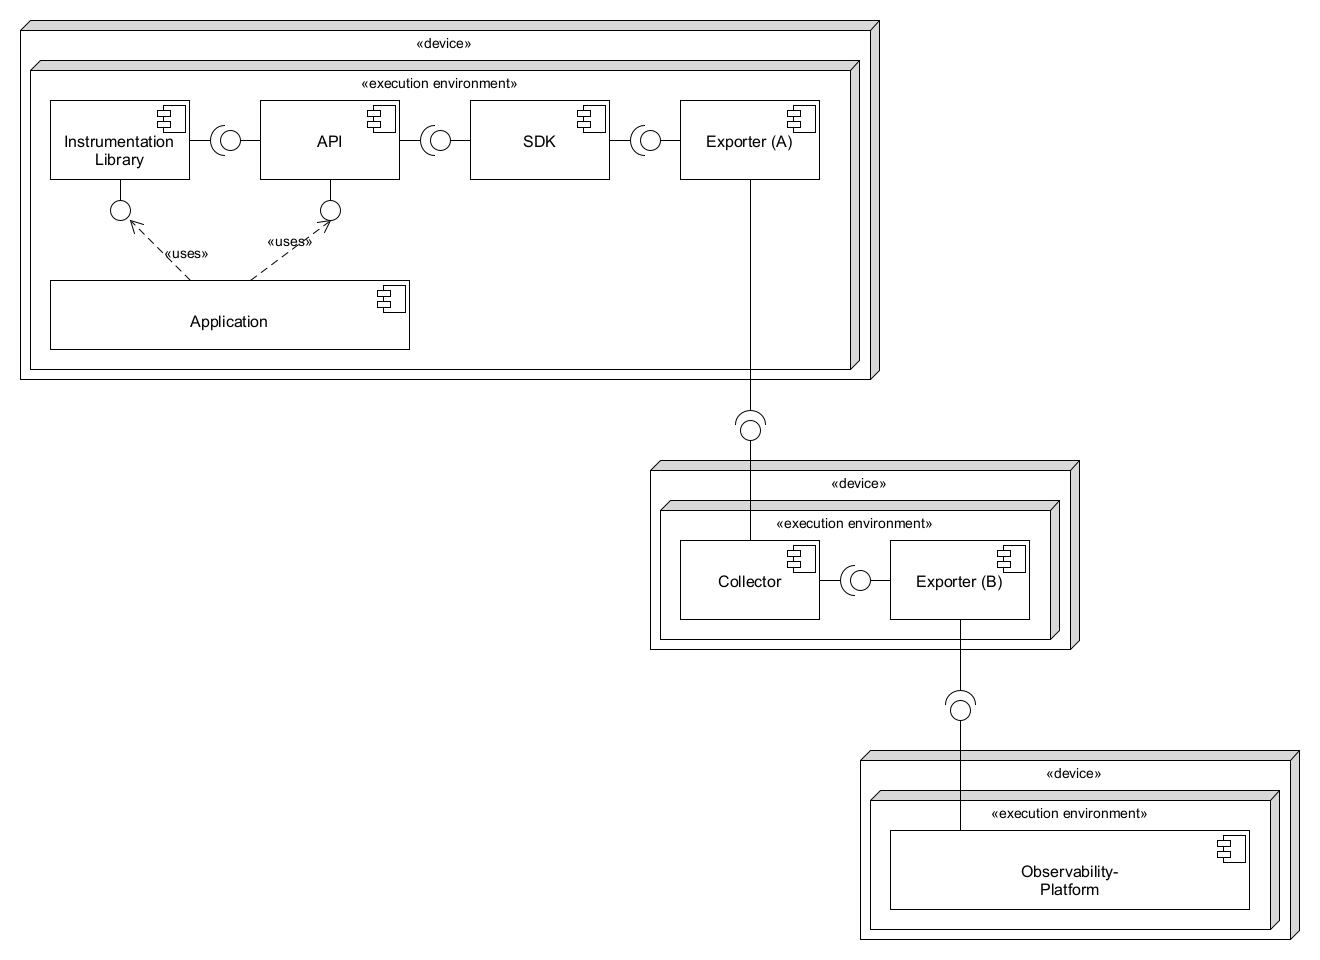
\includegraphics[width=1.00\linewidth]{img/03_methoden/otel_components.png}
	\caption{Komponenten von OpenTelemetry, eigene Darstellung auf Basis von \cite{OTelSpecification}}
	\label{fig:otel-components}
\end{figure}

OpenTelemetry legt somit ein fundiertes Konzept fest, welches die Interoperabilität der derzeit existierenden Systeme erhöhen wird, vorausgesetzt der Standard wird erfolgreich veröffentlicht und auch adaptiert.

%OpenTelemetry (OTel) \cite{OpenTelemetry} ist ein sich derzeit\footnote{Ein erster (General-Availability-)Release der Spezifikation ist für Q1 2021 geplant \cite{OpenTelemetryGARelease}.} entwickelnder herstellerunabhängiger Standard, um Tracing-, Metrik- und Logdaten\footnotemark{} zu erfassen, zu verarbeiten, zu analysieren und zu visualisieren. OTel fasst die beiden Standards OpenTracing und OpenCensus \cite{OpenCensus} zusammen und hat sich als Ziel gesetzt diese zu erweitern \cite{UseNixDistributiveTracing}. Hinter dem Standard stehen u. A. die Cloud Native Computing Foundation (CNCF), Google, Microsoft, und führende Hersteller von Tracing- und Monitoring-Lösungen.
%
%Ziel ist es, dass Entwickler Tools und Werkzeuge benutzen können, ohne erneut hochspezifische Anbindungen schreiben und konfigurieren zu müssen. Stattdessen definiert der Standard Komponenten, die spezielle Aufgabengebiete haben und mit einer allgemeinen API anzusprechen sind. Die technische Infrastruktur einer auf OTel basierenden Lösung ist in \autoref{fig:otel-unified-collection} zu sehen. Im groben definiert OTel folgende Komponenten: API, SDK, Exporter, Collector und Backend (vgl. \autoref{fig:otel-components}).
%
%\nomenclature[Fachbegriff]{OTel}{OpenTelemetry}
%\nomenclature[Fachbegriff]{CNCF}{Cloud Native Computing Foundation}
%\footnotetext{Eine Entwicklung einer Definition zu Logging ist im Gange \cite{OpenTelemetryLoggingSpecification}.}
%
%\begin{figure}[H]
%	\centering
%	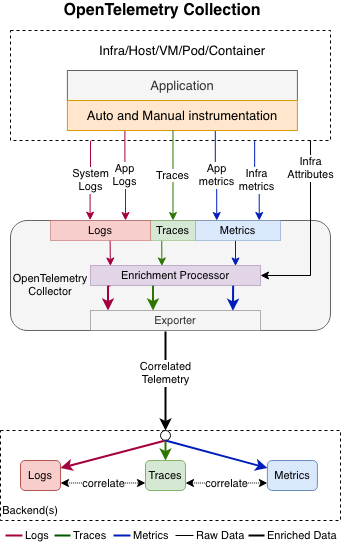
\includegraphics[width=\linewidth]{img/03_methoden/otel_unified-collection_2.png}
%	\caption{Schaubild einer Lösung auf Basis von OTel \cite{OpenTelemetryUnifiedCollection}}
%	\label{fig:otel-unified-collection}
%\end{figure}
%
%\begin{figure}[H]
%	\centering
%	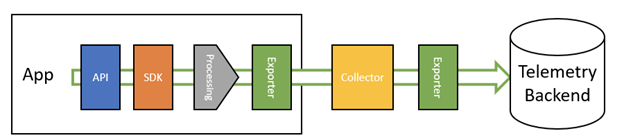
\includegraphics[width=0.75\linewidth]{img/03_methoden/dynatrace_otel-components.png}
%	\caption{OTel Komponenten \cite{DynatraceOTelComponents}}
%	\label{fig:otel-components}
%\end{figure}